\documentclass[
  bibliography=totoc,     % Literatur im Inhaltsverzeichnis
  captions=tableheading,  % Tabellenüberschriften
  titlepage=firstiscover, % Titelseite ist Deckblatt
]{scrartcl}

% Paket float verbessern
\usepackage{scrhack}

% Warnung, falls nochmal kompiliert werden muss
\usepackage[aux]{rerunfilecheck}

% deutsche Spracheinstellungen
\usepackage{polyglossia}
\setmainlanguage{german}

% unverzichtbare Mathe-Befehle
\usepackage{amsmath}
% viele Mathe-Symbole
\usepackage{amssymb}
% Erweiterungen für amsmath
\usepackage{mathtools}

% Fonteinstellungen
\usepackage{fontspec}
% Latin Modern Fonts werden automatisch geladen

\usepackage[
  math-style=ISO,    % ┐
  bold-style=ISO,    % │
  sans-style=italic, % │ ISO-Standard folgen
  nabla=upright,     % │
  partial=upright,   % ┘
  warnings-off={           % ┐
    mathtools-colon,       % │ unnötige Warnungen ausschalten
    mathtools-overbracket, % │
  },                       % ┘
]{unicode-math}

% traditionelle Fonts für Mathematik
\setmathfont{Latin Modern Math}
%\setmathfont{XITS Math}[range={scr, bfscr}]
%\setmathfont{XITS Math}[range={cal, bfcal}, StylisticSet=1]

% Zahlen und Einheiten
\usepackage[
  locale=DE,                 % deutsche Einstellungen
  separate-uncertainty=true, % immer Fehler mit \pm
  per-mode=reciprocal,       % ^-1 für inverse Einheiten
%  output-decimal-marker=.,   % . statt , für Dezimalzahlen
]{siunitx}

% chemische Formeln
\usepackage[
  version=4,
  math-greek=default, % ┐ mit unicode-math zusammenarbeiten
  text-greek=default, % ┘
]{mhchem}

% richtige Anführungszeichen
\usepackage[autostyle]{csquotes}

% schöne Brüche im Text
\usepackage{xfrac}

% Standardplatzierung für Floats einstellen
\usepackage{float}
\floatplacement{figure}{htbp}
\floatplacement{table}{htbp}

% Floats innerhalb einer Section halten
\usepackage[
  section, % Floats innerhalb der Section halten
  below,   % unterhalb der Section aber auf der selben Seite ist ok
]{placeins}

% Seite drehen für breite Tabellen
\usepackage{pdflscape}

% Captions schöner machen.
\usepackage[
  labelfont=bf,        % Tabelle x: Abbildung y: ist jetzt fett
  font=small,          % Schrift etwas kleiner als Dokument
  width=0.9\textwidth, % maximale Breite einer Caption schmaler
]{caption}
% subfigure, subtable, subref
\usepackage{subcaption}

% Grafiken können eingebunden werden
\usepackage{graphicx}
% größere Variation von Dateinamen möglich
\usepackage{grffile}

% schöne Tabellen
\usepackage{booktabs}

% Verbesserungen am Schriftbild
\usepackage{microtype}

% Literaturverzeichnis
\usepackage[
  backend=biber,
]{biblatex}
% Quellendatenbank
\addbibresource{../lit.bib}
\addbibresource{../latex-template/programme.bib}

% Hyperlinks im Dokument
\usepackage[
  unicode,        % Unicode in PDF-Attributen erlauben
  pdfusetitle,    % Titel, Autoren und Datum als PDF-Attribute
  pdfcreator={},  % ┐ PDF-Attribute säubern
  pdfproducer={}, % ┘
]{hyperref}
% erweiterte Bookmarks im PDF
\usepackage{bookmark}

% Trennung von Wörtern mit Strichen
\usepackage[shortcuts]{extdash}

\author{
  Ann-Sophie Schubert%
  \texorpdfstring{
    \\
    \href{mailto:ann-sophie.schubert@udo.edu}{ann-sophie.schubert@udo.edu}
  }{}%
  \texorpdfstring{\and}{, }
  Lars Funke
  \texorpdfstring{
    \\
    \href{mailto:lars.funke@udo.edu}{lars.funke@udo.edu}
  }{}%
}
\publishers{TU Dortmund – Fakultät Physik}

\subject{201}
\title{Das Dulong-Petitsche Gesetz}
\date{
  Durchführung: 26.01.2016
  \hspace{3em}
  Abgabe: 29.01.2016
}

\begin{document}

\maketitle
\newpage
\mbox{}
\newpage
\thispagestyle{empty}
\tableofcontents
\newpage

\section{Theorie}
\label{sec:Theorie}

Ein Lock-In-Verstärker wird benutzt, um (stark) verrauschte periodische Signale zu verstärken und zu messen. Dazu wird das Signal, welches zuvor durch einen Bandpassfilter von höher- ($\omega \gg \omega_0$) und niederfrequentem ($\omega \ll \omega_0$) Rauschen befreit wurde mit einem Referenzsignal moduliert. Dieses kann durch einen Phasenschieber an das zu messende Signal angeglichen werden, sodass die Schwinugen in Phase sind ($\Delta \phi = 0$). Zuletzt wird das Mischsignal mit einem Tiefpassfilter über mehrere Perioden aufintegriert, wobei sich die stochastischen Rauschanteile bei ausreichender Zeitkonstante $\tau = RC \gg \sfrac{1}{\omega_0}$ aufheben.

\begin{figure}
  \centering
  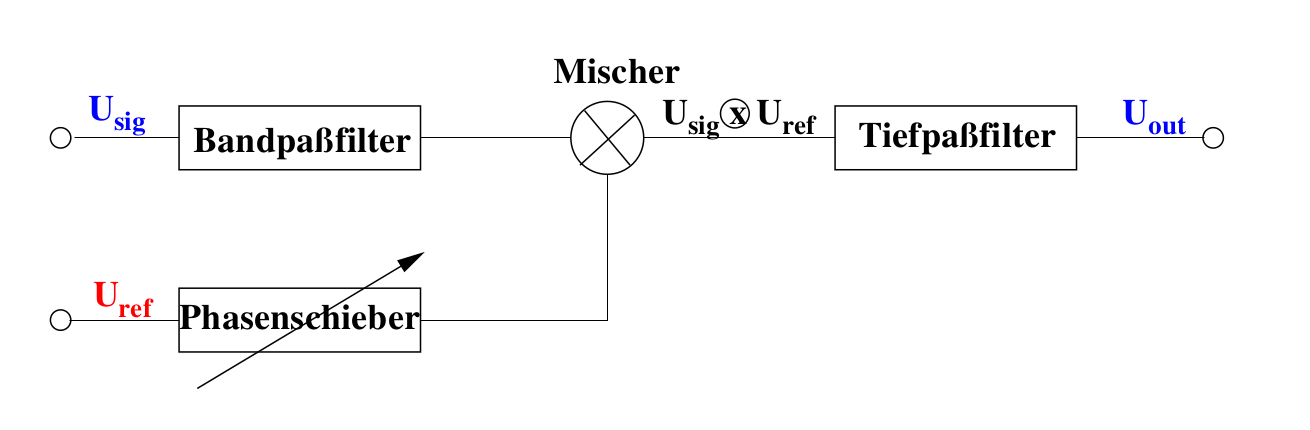
\includegraphics[width=\textwidth]{content/grafiken/Schema.png}
  \caption{Schematische Darstellung eines Lock-In-Verstärkers}
  \label{fig:schema}
\end{figure}

\begin{figure}
  \centering
  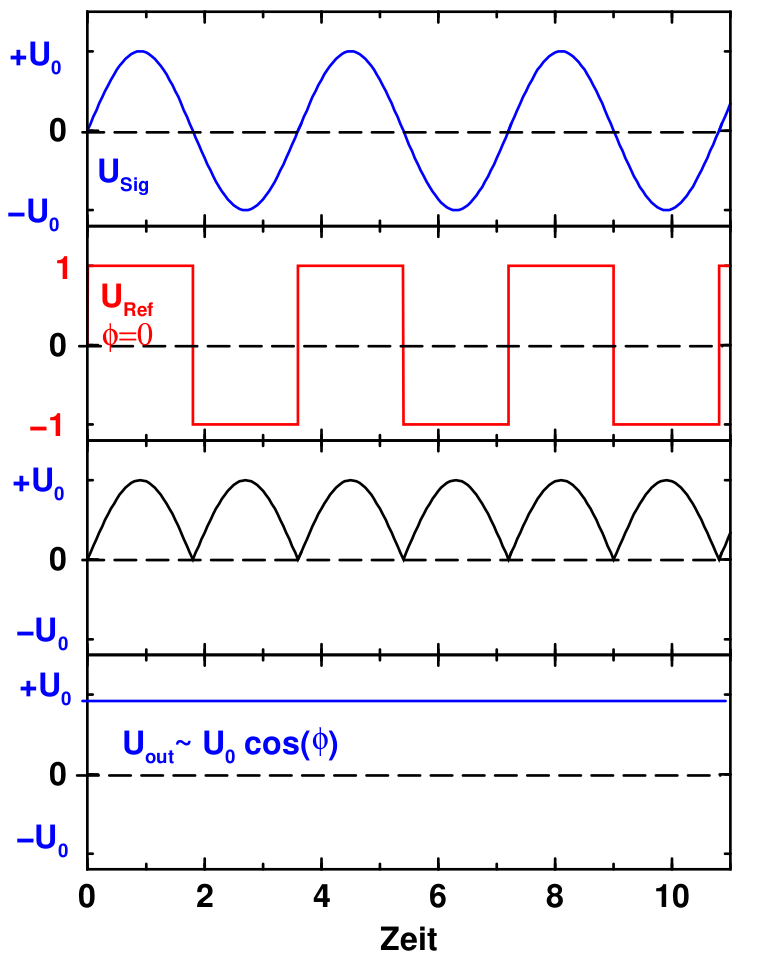
\includegraphics[width=.5\textwidth]{content/grafiken/Wellen.png}
  \caption{Schematische Darstellung eines Lock-In-Verstärkers}
  \label{fig:wellen}
\end{figure}

Für eine sinusförmige Spannung
\begin{equation}
  U_\mathrm{sig} = U_0 \cdot \sin (\omega t),
\end{equation}
welche mit einer synchronisierten Rechteckspannung $U_\mathrm{ref}$ der Amplitude $1$ moduliert wird, ergibt sich, wie in Abb.~\ref{fig:wellen} ersichtlich nach der Modulation ein Signal welches dem Betrag der Signalspannung entspricht. Die unteren Halbwellen wurden also an der Zeitachse gespiegelt.
Zur Bestimmung der Ausgangsspannung wird nun das Referenzsignal mit einer Fourier-Reihe genähert, sodass
\begin{equation}
  U_\mathrm{ref} = \frac{4}{\pi} \left( \sin(\omega t) + \frac{1}{3} \sin(3\omega t) + \frac{1}{5} \sin(5\omega t) + … \right)
\end{equation}
ist. Das Produkt des Signals mit der Referenzschwingung, also das modulierte Signal hat somit die Schwingungsgleichung
\begin{equation}
  U_\mathrm{sig} \times U_\mathrm{ref} = \frac{2}{\pi} U_0 \left( 1 - \frac{2}{3} \sin(2 \omega t) + \frac{2}{15} \sin(4\omega t) + \frac{2}{35} \sin(6\omega t) + … \right).
\end{equation}
Durch den Tiefpassfilter werden zuletzt die Schwingungsanteile entfernt und übrig bleibt nur die Ausgangsspannung
\begin{equation}
  U_\mathrm{out} = \frac{2}{\pi} U_0.
\end{equation}
Sind $U_\mathrm{ref}$ und $U_\mathrm{sig}$ nicht in Phase, sondern mit einer Phasenschiebung $\phi$ versehen, ist die Ausgangsspannung von dieser abhängig:
\begin{equation}
  U_\mathrm{out} = \frac{2}{\pi} U_0 \cos \phi
\end{equation}

\section {Aufbau und Durchführung}
\label{sec:durchführung}
\subsection{Messung der Gegenstandsweite und Bildweite}
Bei fester Gegenstandsweite $g$ wird der Schirm so lange verschoben, bis auf diesem ein scharfes Bild erkennbar ist. Dies wird für 10 verschiedene Gegenstandsweiten wiederholt und dazugehörige Bildweite $b$ wird aufgenommen.

\subsection{Methode von Bessel}
\fig{bilder/bessel.pdf}{Schematischer Aufbau zur Bestimmung der Brennweite mit der Methode von Bessel \cite{anleitung408}.}{Bessel}
In Abbildung \ref{fig:Bessel} ist der Aufbau für die Methode von Bessel schematisch dargstellt. Hier ist der Abstand $e$ zwischen Gegenstand und Schirm fest. Die Position der Linse wird so verändert, dass auf dem Schirm ein scharfes Bild zu sehen ist. Die Werte für die Bildweite $b_1$ und die Gegenstandeite $g_1$ werden notiert. Dann wird die Linse erneut verschoben, bis ein scharfes Bild auf dem Schirm erkennbar ist. Erneut werden die zugehörigen Werte $b_2$ und $g_2$ aufgenommen.
Es gelten folgende Zusammenhänge:
\begin{align}
  b_1 &= g_2 \\
  b_2 &= g_1 \\
  e &= g_1+b_1 =g_2+b_2 \\
  d &= g_1 - b_1 = g_2 -b_2
\end{align}
Daraus lässt sich die Brennweite $f$ berechnen:
\begin{equation}
  f = \frac{e^2 - d^2}{4e}
\end{equation}

Die Messung wird für insgesamt 10 verschiedene Abstände $e$ zwischen Gegenstand und Schirm durchgeführt.

Zusätzlich soll die chromatische Aberration betrachtet werden. Dazu wird einmal ein blauer und einmal ein roter Filter eingesetzt und der zuvor erläuterte Messvorgang für jeweils 5 Abstände $e$ zwischen Gegenstand und Schirm durchgeführt.

\subsection{Methode von Abbe}
\fig{bilder/abbe.pdf}{Schematischer Aufbau zur Bestimmung der Brennweite mit der Methode von Abbe \cite{anleitung408}.}{abbe}
Wie Abbildung \ref{fig:abbe} zeigt, besteht der Aufbau aus einer Sammel- und einer Zerstreuungslinse. Hier soll die Brennweite des Linsensystems ermittelt werden. Über den Abbildungsmaßstab $V$ kann sowohl die Brennweite als auch die Lage der Hauptebenen bestimmt werden. Es wird ein beliebiger Referenzpunkt $A$ ausgesucht, weil nicht bekannt ist, wo die Hauptebenen liegen. Die Längen $b'$ und $g'$ sind die gemessene Bild- beziehungsweise Gegenstandsweite. Damit kann der Brennpunkt und die Position der Hauptebenen ermittelt werden.
\begin{align}
  g' &= g + h = f \cdot\left( 1+\frac{1}{V}\right)+h\\
  b' &= b + h' = f \cdot (1 + V) + h'
\end{align}

Die Messung wird für 10 Gegenstandsweiten durchgeführt.

\section{Auswertung}
\label{sec:Auswertung}

%\section{Fehlerrechnung}
\label{subsec:fehlerrechnung}

\subsubsection{Mittelwert}
\begin{equation}
\overline{v} = \frac{1}{N} \sum_{i=1}^N v_i
\end{equation}

\subsubsection{Standardabweichung}
\begin{equation}
s_i = \sqrt{\frac{1}{N - 1} \sum_{j=1}^N \left(v_j - \overline{v}\right){^2}}
\end{equation}

wobei $v_j$ ($j = 1, ..., N$) die Messwerte sind.

\subsubsection{Streuung der Mittelwerte}
\begin{equation}
\sigma_i = \frac{s_i}{\sqrt{N}} = \sqrt{\frac{\sum_{j=1}^N \left(v_j - \overline{v_i}\right){^2}}{N \left(N - 1 \right)}}
\end{equation}

\subsubsection{Gaußfehler}
Bei einer fehlerbehafteten Funktion $f$ mit $k$ als fehlerbehafteter Größe und $\sigma_k$ als Ungenauigkeit, gilt:

\begin{equation}
\Delta x_k = \frac{\mathrm{d}f}{\mathrm{d}k}\sigma_k
\end{equation}.

 Der relative Gaußfehler berechnet sich nach:
\begin{equation}
\Delta x_\text{k, rel} = 1 \pm \frac{\Delta x_k}{|x|}\cdot 100\%
\end{equation}.

Der absolute Gaußfehler ergibt sich aus:
\begin{equation}
\Delta x_i = \sqrt{\left(\frac{\mathrm{d}f}{\mathrm{d}k_{1}}\cdot \sigma_{k_{1}}\right)^2 + \left(\frac{\mathrm{d}f}{\mathrm{d}k_{2}}\cdot \sigma_{k_{2}}\right)^2 + ...}
\end{equation}.


\subsection{Auf- und Entladevorgang}
\label{sec:a}
Die Zeitkonstante $\tau = RC$ eines RC-Kreises wird Anhand der Auf-/Entladekurve bestimmt. Dazu wird ein Stromkreis wie in Abb. \ref{fig:rc-kreis} genutzt, wobei $U_C$ mit einem digitalen Speicheroszilloskop gemessen wird. Der gemessene Spannungsverlauf findet sich in Abb. \ref{fig:entladekurve}.
\begin{figure}
  \centering
  \includegraphics{build/a1.pdf}
  \caption{Verlauf der Kondensatorspannung $U_C$ bei angelegter Rechteckspannung am RC-Kreis. Zur Bestimmung der Zeitkonstante wird der mit den schwarzen vertikalen Linien markierte Zeitbereich genutzt.}
  \label{fig:entladekurve}
\end{figure}
Zur Auswertung wird nun das Spannungsoffset
\begin{equation}
  U_0 = \SI{-5.6}{\volt}
\end{equation}
korrigiert, die Messwerte logarithmiert und mittels linearer Regression die Steigung einer Ausgleichsgeraden ermittelt. Aus (\ref{a}) folgt über
\begin{align}
  U (t) &= U (0) \cdot \symup{e}^{\sfrac{-t}{RC}}\\
  \ln{U(t)} &= \ln{(U (0) \cdot \symup{e}^{\sfrac{-t}{RC}})} \\
  \ln{U(t)} &= \ln{U (0)} - \frac{1}{RC} \cdot t
\end{align}

, dass

\begin{equation}
  RC = -\frac{1}{a}
\end{equation}

ist, mit der Steigung $a$ der Ausgleichsgeraden. Die logarithmierten Messwerte über die Zeit aufgetragen finden sich in Abb. \ref{fig:auswertung_a}, das Ergebnis lautet
\begin{equation}
  RC = \SI{1.360+-0.001}{\milli\second}
\end{equation}
%\begin{table}
%  \centering
%  \caption{Ergebnis der Auswertung der Zeitkonstante des RC-Kreises.}
%  \label{tab:ergebnis_a}
%  \sisetup{
%    round-mode=figures
%  }
%  \begin{tabular}{
%    l@{}
%    S[table-format=1.3e2, round-precision=4] @{${}\pm{}$} S[table-format=1.2e2, round-precision=3]
%  }
%    \toprule
%    & \multicolumn{2}{c}{RC / \si{\second}} \\
%    \midrule
%    \begin{table}
        \caption{Messergebnisse aus dem A-Scan. Neben den abgelesenen und berechneten Daten $d_n$ sind auch die zuvor mittels Messschieber bestimmten Abmessungen $d_n^\text{mech}$ eingetragen.}
        \centering
        \label{tab:a}
        \begin{tabular}{l@{}S[round-mode=off, table-format=2.0]S[table-format=2.3, round-precision=4, round-mode=off] S[table-format=2.2, round-precision=4, round-mode=figures] S[table-format=1.4, round-precision=4, round-mode=figures] S[table-format=2.3, round-precision=4, round-mode=figures] S[table-format=2.2, round-precision=4, round-mode=figures] S[table-format=2.4, round-precision=4, round-mode=off] } \toprule & {$\text{Störstelle}$}& {$d_1/\si{mm}$}& {$d_2/\si{mm}$}& {$2r/\si{mm}$}& {$d_1^\text{mech}/\si{mm}$}& {$d_2^\text{mech}/\si{mm}$}& {$2r^\text{mech}/\si{mm}$}\\\midrule
& 1 & 18.02 & 61.56149999999999522515 & 0.46050000000000257394 & 19.62000000000000099476 & 59.61999999999999744205 & 0.80 \\
& 2 & 19.93 & 59.78699999999999192823 & 0.32400000000000828138 & 17.76000000000000156319 & 61.29999999999999715783 & 0.98 \\
& 3 & 61.29 & 13.78650000000000019895 & 4.96500000000000429878 & 61.28000000000000113687 & 13.43999999999999950262 & 5.32 \\
& 4 & 54.05 & 22.11299999999999599254 & 3.87300000000000821387 & 53.84000000000000341061 & 21.69999999999999928946 & 4.50 \\
& 5 & 46.68 & 30.43950000000000244427 & 2.91749999999998976818 & 46.50000000000000000000 & 30.07999999999999829470 & 3.46 \\
& 6 & 39.04 & 39.03900000000000147793 & 1.96199999999999152855 & 38.60000000000000142109 & 38.71999999999999886313 & 2.72 \\
& 7 & 31.12 & 47.09249999999999403144 & 1.82550000000000767209 & 30.82000000000000028422 & 46.88000000000000255795 & 2.34 \\
& 8 & 23.07 & 55.14600000000000079581 & 1.82550000000000411937 & 22.78000000000000113687 & 54.82000000000000028422 & 2.44 \\
& 9 & 15.01 & 62.92650000000001142553 & 2.09849999999999115019 & 14.82000000000000028422 & 62.97999999999999687361 & 2.24 \\
& 10 & 7.23 & 70.98000000000000397904 & 1.82549999999999990052 & 6.87999999999999989342 & 70.79999999999999715783 & 2.36 \\
& 11 & 55.82 & 15.42450000000000009948 & 8.78699999999999548095 & 55.11999999999999744205 & 14.63000000000000078160 & 10.29 \\
 \bottomrule \end{tabular} \end{table}

%    \bottomrule
%  \end{tabular}
%\end{table}

\begin{figure}
  \centering
  \includegraphics{build/a2.pdf}
  \caption{Logarithmierter Kondensatorspannungsverlauf mit Ausgleichsgerade. Fehlerbalken wurden zur Verbesserung der Lesbarkeit ausgelassen.}
  \label{fig:auswertung_a}
\end{figure}

\subsection{Schwingungsverhalten}
\label{sec:b}
Nun soll die Zeitkonstante auf andere Art und Weise ermittelt werden, undzwar dadurch, dass eine Wechselspannung an den RC-Kreis angelegt wird und dabei die resultierende Spannung bzw. Phasenverschiebung gemessen wird. Der Aufbau der Schaltung findet sich an Abb. \ref{fig:phase-frequenz}. Hierbei wird die Zeitkonstante mittels nichtlinearer Ausgleichsrechnung an die der Formeln (\ref{eqn:amplitude}) und (\ref{eqn:phase}) bestimmt. Die Ergebnisse finden sich in Tabelle \ref{tab:ergebnis_b} und Abb. \ref{fig:auswertung_b1}/\ref{fig:auswertung_b2}.

\begin{table}
  \centering
  \caption{Ergebnis der Auswertung der Zeitkonstante des RC-Kreises.}
  \label{tab:ergebnis_b}
  \sisetup{
    round-mode=figures
  }
  \begin{tabular}{
    l
    S[table-format=1.2e2, round-precision=3] @{${}\pm{}$} S[table-format=1.0e2, round-precision=1]
  }
    \toprule
    & \multicolumn{2}{c}{RC / \si{\second}} \\
    \midrule
    Messreihe Amplitude \input{build/b1.txt}
    Messreihe Phasenverschiebung \input{build/b2.txt}
    \bottomrule
  \end{tabular}
\end{table}

\begin{figure}
  \centering
  \includegraphics{build/b1.pdf}
  \caption{Frequenzabhängigkeit des Verhältnisses der Amplitude am Kondensator zur angelegten Amplitude, einfachlogarithmische Darstellung.}
  \label{fig:auswertung_b1}
\end{figure}

\begin{figure}
  \centering
  \includegraphics{build/b2.pdf}
  \caption{Frequenzabhängigkeit der Phasenverschiebung von Kondensator- und Generatorspannung, einfachlogarithmische Darstellung.}
  \label{fig:auswertung_b2}
\end{figure}

\newpage
\subsection{Integrator}
\label{sec:c}
Bei ausreichend hohen Frequenzen $\omega \gg \sfrac{1}{RC}$ kann ein RC-Kreis als Integrationsglied verwendet werden. Die hochfrequenten Anteile der angelegten Spannung werden dabei aufintegriert. Einige Beispiele dazu finden sich in den Abbildungen \ref{fig:d1}, \ref{fig:d2} und \ref{fig:d3}.

\begin{figure}
  \centering
  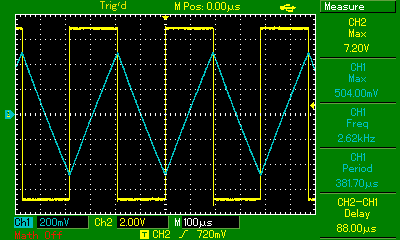
\includegraphics[scale=0.8]{daten/d/MAP004.png}
  \caption{Spannungsverlauf einer Dreiecksschwingung und der vom RC-Kreis integrierten resultierenden Parabelschwingung.}
  \label{fig:d1}
\end{figure}

\begin{figure}
  \centering
  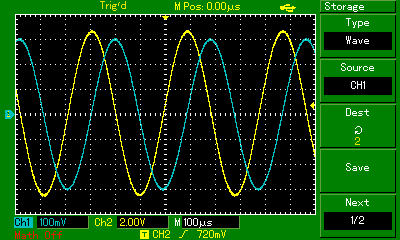
\includegraphics[scale=0.8]{daten/d/MAP005.png}
  \caption{Spannungsverlauf einer Rechteckschwingung und der vom RC-Kreis integrierten resultierenden Dreieckschwingung.}
  \label{fig:d2}
\end{figure}

\begin{figure}
  \centering
  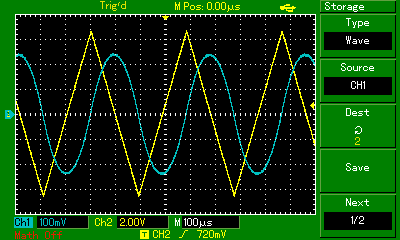
\includegraphics[scale=0.8]{daten/d/MAP006.png}
  \caption{Spannungsverlauf einer Sinusschwingung und der vom RC-Kreis integrierten resultierenden Cosinusschwingung.}
  \label{fig:d3}
\end{figure}

\subsection{Messdaten}
Die Angabe der Oszilloskop-Messdaten aus \ref{sec:a} ist aufgrund der Menge (6000 Punkte) nicht möglich. Die restlichen Daten finden sich in Tabelle \ref{tab:daten}.

\begin{table}
  \centering
  \caption{Messdaten.}
  \label{tab:daten}
  \sisetup{
    round-mode=figures
  }
  \begin{tabular}{
      l@{}
      S[table-format=5.0]
      S[table-format=1.3]
      S[table-format=1.1]
      S[round-precision=3, table-format=1.4] @{${}\pm{}$} S[round-precision=2, table-format=1.5]
      S[table-format=1.2]
      S[round-precision=3, table-format=1.4] @{${}\pm{}$} S[round-precision=2, table-format=1.4]
    }
    \toprule
    & {$f / \si{\hertz}$} & {$U/ \si{\volt}$} & {$U_0 / \si{\volt}$} & \multicolumn{2}{c}{A} & {$a / \si{\milli\second}$} & \multicolumn{2}{c}{$\phi / \si{\radian}$}\\
    \midrule
    \input{build/daten.txt}
    \midrule
    &\multicolumn{8}{c}{
      $\Delta U^\text{rel} = 5\%, \quad \Delta U_0^\text{rel} = 5\%, \quad \Delta a^\text{rel} = 5\%$
    }\\
    \bottomrule
  \end{tabular}
\end{table}

\section{Diskussion}
\label{sec:Diskussion}

Die Abweichung des Schubmoduls um $(21,8 \pm 0,009)\%$ liegt innerhalb des Toleranzbereiches, da es mehrere Messunsicherheiten gibt, die nicht weiter berücksichtigt werden. Zum Einen wird das Schwingen des Pendels durch Bewegung des Tisches, wie zum Beispiel leichtes Anstoßen beeinflusst. Außerdem kann der Magnet nicht exakt in Nord-Süd Richtung ausgerichtet werden, sodass das Erdmagnetfeld die Messung trotz dieser Einrichtung beeinflusst. Weiterhin ist zu beachten, dass die in der Theorie angenomme Kleinwinkelnäherung nicht immer angehalten wurde, was zu weiterem Fehlern führt.



\nocite{numpy}
\nocite{matplotlib}
\nocite{uncertainties}
\printbibliography

\end{document}
